\subsection{Informacije o isporuci za dostavljača}

Ako dostavljač klikne na neku od zakazanih dostava prikazuju mu se detaljnije informacije o toj dostavi (slika \ref{fig:DeliverymanOrderInfo}).
Ako dostavljač kasni ovde ima mogućnost da obavesti klijenta o tome. Kada se klikne na "Notify about the delay" pojavljuje se forma (slika \ref{fig:DeliverymanDelay}) gde bi trebalo da ukuca njegovu procenu koliko će kasniti. Sistem automatski šalje poruku korisniku i obaveštava ga o kašnjenju.
Kada dostavu završi potrebno je da klikne dugme "Delivered". Nakog toga sistem čuva da je ova porudžbina dostavljena a dostavljaču se prikazuje poruka koja mu čestita na obavljenoj dostavi i nudi mu mogućnost da se vrati na preostale isporuke (slika \ref{fig:DeliverymanDone}). Kada se vrati na ekran sa listom svih isporuka, završena dostava je obrisana (slika \ref{fig:DeliverymanDone}).


\begin{figure}[H]
	\begin{center}
		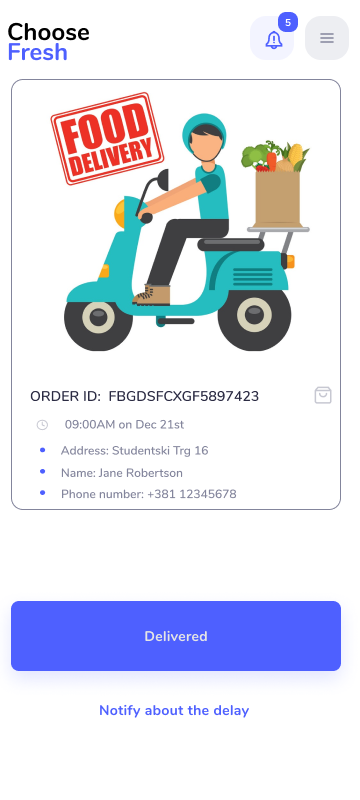
\includegraphics[scale=0.3]{UI/deliveryman_order_info.png}
    		\caption{Ekran informacija o isporuci za dostavljača}
    \label{fig:DeliverymanOrderInfo}
    \end{center}
\end{figure}

\begin{figure}[H]
	\begin{center}
		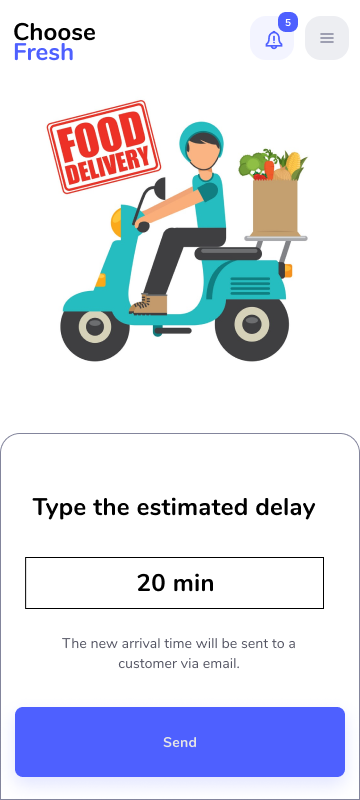
\includegraphics[scale=0.3]{UI/deliveryman_delay_input.png}
    		\caption{Ekran za obaveštavanje klijenta o kašnjenju}
    \label{fig:DeliverymanDelay}
    \end{center}
\end{figure}

\begin{figure}[H]
	\begin{center}
		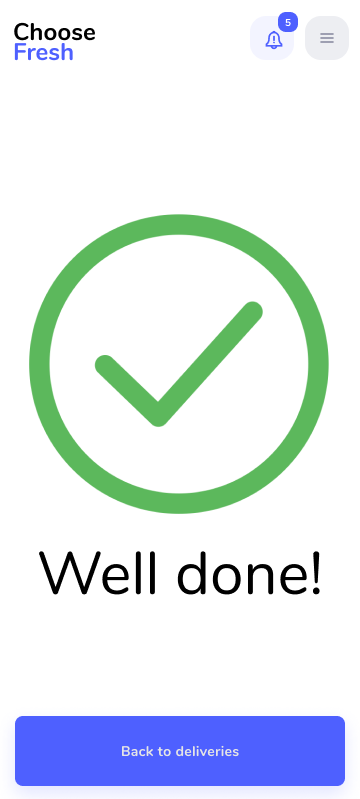
\includegraphics[scale=0.3]{UI/deliveryman_done_delivery.png}
    		\caption{Ekran poruke nakon obavljene dostave}
    \label{fig:DeliverymanDone}
    \end{center}
\end{figure}

\begin{figure}[H]
	\begin{center}
		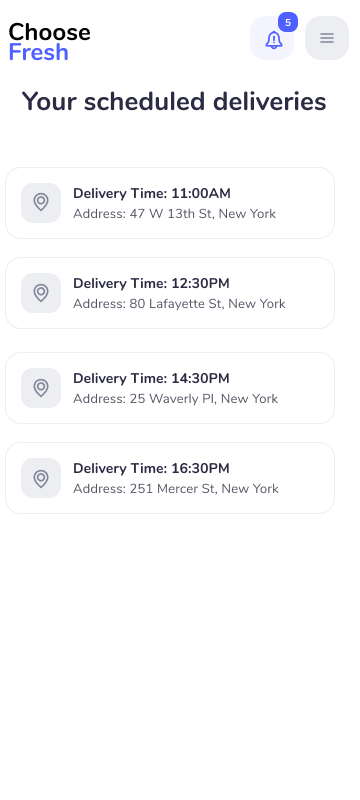
\includegraphics[scale=0.3]{UI/deliveryman_list_of_packages_new.png}
    		   \caption{Ekran liste zakazanih isporuka dostavljača nakon dostavljanja prve isporuke}
    \label{fig:DeliverymanListNew}
    \end{center}
\end{figure}